\clearpage

\section {Difference between sin$^{2}\theta_{23}$  values for maximal mixing and maximal disappearance.}
\label{app:symmetry}

%As it has been already shown in this note, for instance in figures \ref{fig:mirrordef} or \ref{fig:1Dchisqtheta23}, 

As it has been already shown in this note,  $\Delta\chi^2$ is not always symmetric with respect to sin$^{2}\theta_{23}$ = 0.5. 
The reason for this behaviour will be explained in this section. 

The distribution of $\Delta\chi^{2}$ vs $\sin^{2}\theta_{23}$ has two minima which are at values of $\sin^{2}\theta_{23}$ that are symmetric 
with respect to a center of symmetry (see, for example, figure \ref{fig:toymc1_dchisq_sinsqtheta23}). It seems natural to think that 
this center of symmetry must be at exactly $\sin^{2}\theta_{23}$ = 0.5 since the value of $\sin^{2}2\theta_{23}$ is exactly identical for 
$\theta_{23}$ and $\pi/2-\theta_{23}$. However it will be shown in this section that the position of the center of symmetry depends on the value 
of $\sin^{2}\theta_{13}$ and that it is at 0.5 only if $\sin^{2}\theta_{13}$ = 0. 

All the results in this technical note include matter effects, but the following calculation is made using the 3-flavour vacuum oscillation 
probabilities so that the algebra is manageable:

%In the 2-flavour approximation, the oscillation probabilities can be written as:

%\begin{equation}
%\begin{array}{c}
%P(\nu_{\mu}\rightarrow\nu_{\mu}) = 1 - sin^{2}2\theta_{23} sin^{2} \left(  \frac{\Delta m_{32}^{2} L}{4E_{\nu}}\right) \\
%P(\nu_{\mu}\rightarrow\nu_{e}) = sin^{2}2\theta_{13}sin^{2}\theta_{23} sin^{2} \left(  \frac{\Delta m_{31}^{2} L}{4E_{\nu}}\right)
%\end{array}
%\label{eq:2f}
%\end{equation}

%In this particular case the oscillation probability $P(\nu_{\mu}\rightarrow\nu_{\mu})$ only depends on $sin^{2}2\theta_{23}$ and therefore the distribution of oscillation probability will be symmetric with respect to $sin^{2}2\theta_{23}=0.5$. However, this is not valid any more as long as the 2 flavour approximation is abandoned to use a complete 3 flavour oscillation probability and $sin^{2}\theta_{13}\neq0$.

%Let's take now the 3 flavour oscillation probability (matter effects will be neglected in the following calculations as they are very small for T2K):

\begin{equation}
\begin{array}{r}
P(\nu_{\alpha}\rightarrow\nu_{\beta}) = \delta_{\alpha\beta} - 4 \displaystyle\sum_{i>j} \mathcal{R}e \left[ U_{\alpha i}^{*}U_{\beta i}U_{\alpha j} U_{\beta j}^{*} \right] sin^{2}\left(\frac{\Delta m_{ij}^{2} L}{4E}\right)\\
+2\displaystyle\sum_{i>j} \mathcal{I}m \left[ U_{\alpha i}^{*}U_{\beta i}U_{\alpha j} U_{\beta j}^{*} \right] sin\left(\frac{\Delta m_{ij}^{2} L}{2E}\right)
\end{array}
\label{eq:nuanub3foscprob}
\end{equation}
where $U_{ab}$ represents the ab element of the PMNS matrix:

\begin{equation}
U = \left(
\begin{array}{ccc}
c_{12}c_{13} & c_{13}s_{12} & s_{13}e^{-i\delta} \\
-c_{23}s_{12} - s_{13}s_{23}c_{12}e^{i\delta} & c_{12}c_{23} - s_{12}s_{13}s_{23}e^{i\delta} & c_{13}s_{23} \\
s_{12}s_{23} - s_{13}c_{12}c_{23}e^{i\delta} & -s_{23}c_{12} - s_{12}c_{23}s_{13}e^{i\delta} & c_{13}c_{23}
\end{array} \right)
\label{eq:PMNSmatrix}
\end{equation}
with $s_{12} = \sin(\theta_{12})$, $c_{12} = \cos(\theta_{12})$, etc. 

The $\nu_{\mu}$-survival probability is plotted as a function of $\sin^{2}(\theta_{23})$ in figure \ref{fig:oscprobdifftheta13} for different values 
of $\sin^{2}(\theta_{13})$. From this figure, it can be seen that the center of symmetry is only at $\sin^{2}(\theta_{23})$ = 0.5 for 
$\sin^{2}(\theta_{13})$ = 0 and that it moves to higher values of $\sin^{2}(\theta_{23})$ as $\sin^{2}(\theta_{13})$ increases, for both mass hierarchies.
The center of symmetry of the P($\nu_{\mu}\rightarrow\nu_{\mu}$) curve corresponds to its minimum and therefore to the maximal disappearance,
so both terms, center of symmetry of the P($\nu_{\mu}\rightarrow\nu_{\mu}$) curve and maximal disappearance are equivalent.

%\begin{figure}[htbp]
%\begin{center}
%\includegraphics[width=0.5\textwidth]{images/appendix/NuMuOscProbVacuumSeveralValuesMix13Normal.eps}\includegraphics[width=0.5\textwidth]{images/appendix/NuMuOscProbMatterSeveralValuesMix13Normal.eps}
%\caption{Comparison of 90\% (blue) and 68\% (red) C.L. contours for the official $\nu_{e}$-appearance analysis \cite{NueRun1and2Analysis} (dashed, light colors)  and the ones obtained with the framework used in this work (solid, dark colors). The new contours are in good agreement with the official ones, small differences appear due to the limited number of FC jobs run for this comparison.}
%\label{fig:nuecomparison}
%\end{center}
%\end{figure}

The 3-flavour $\nu_{\mu}$-survival probability is


\begin{figure}[htbp]
\begin{center}
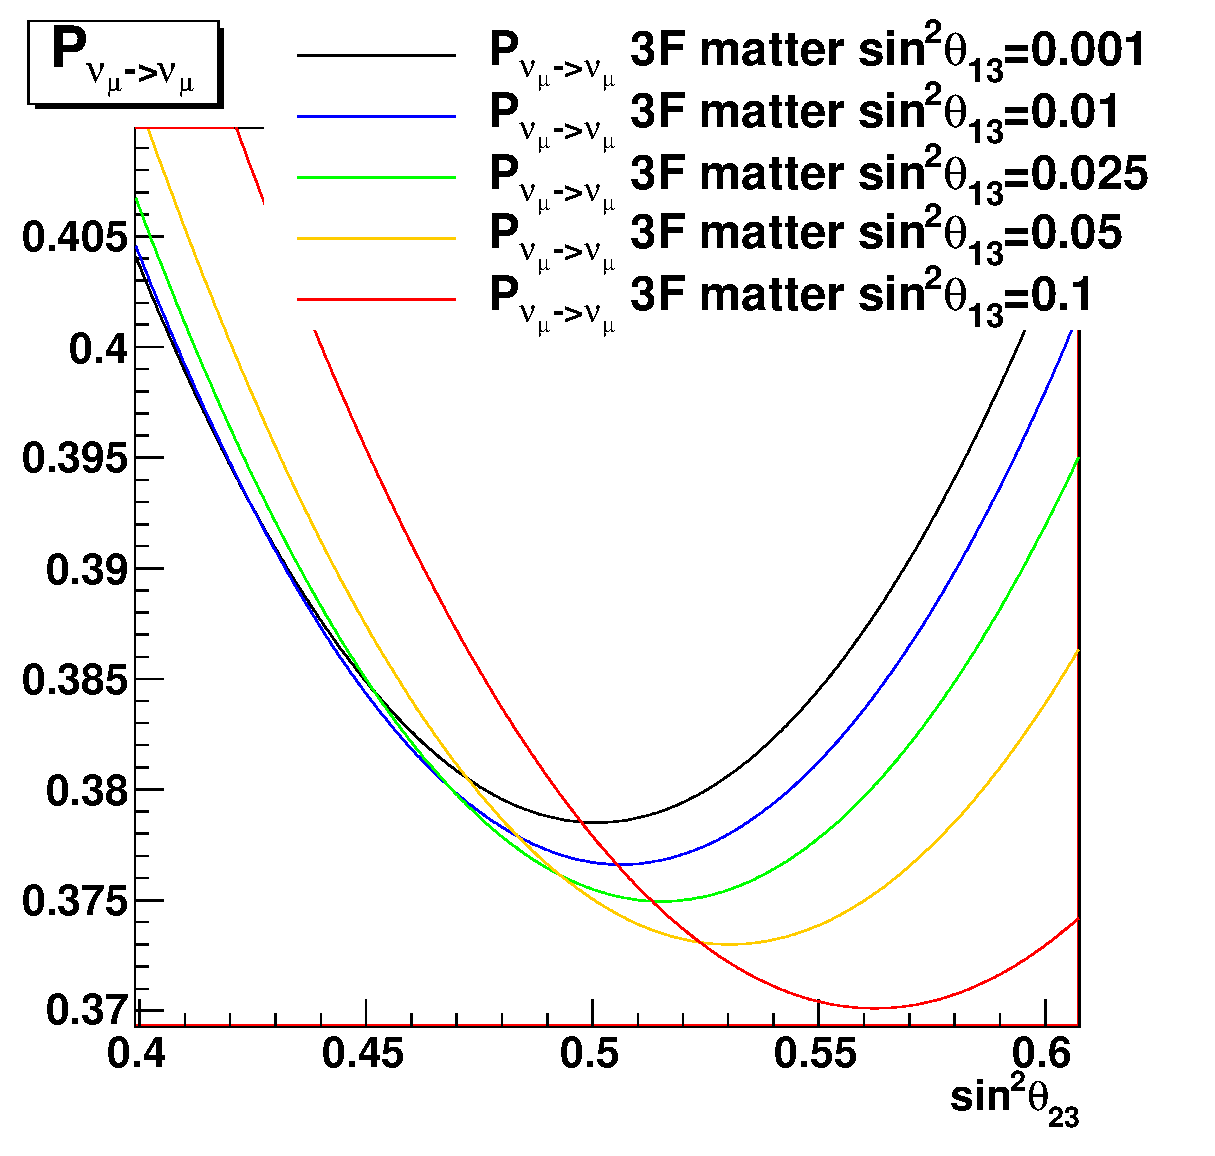
\includegraphics[width=0.5\textwidth]{images/appendix/theta23_symmetry/NuMuOscProbMatterSeveralValuesMix13Normal.eps}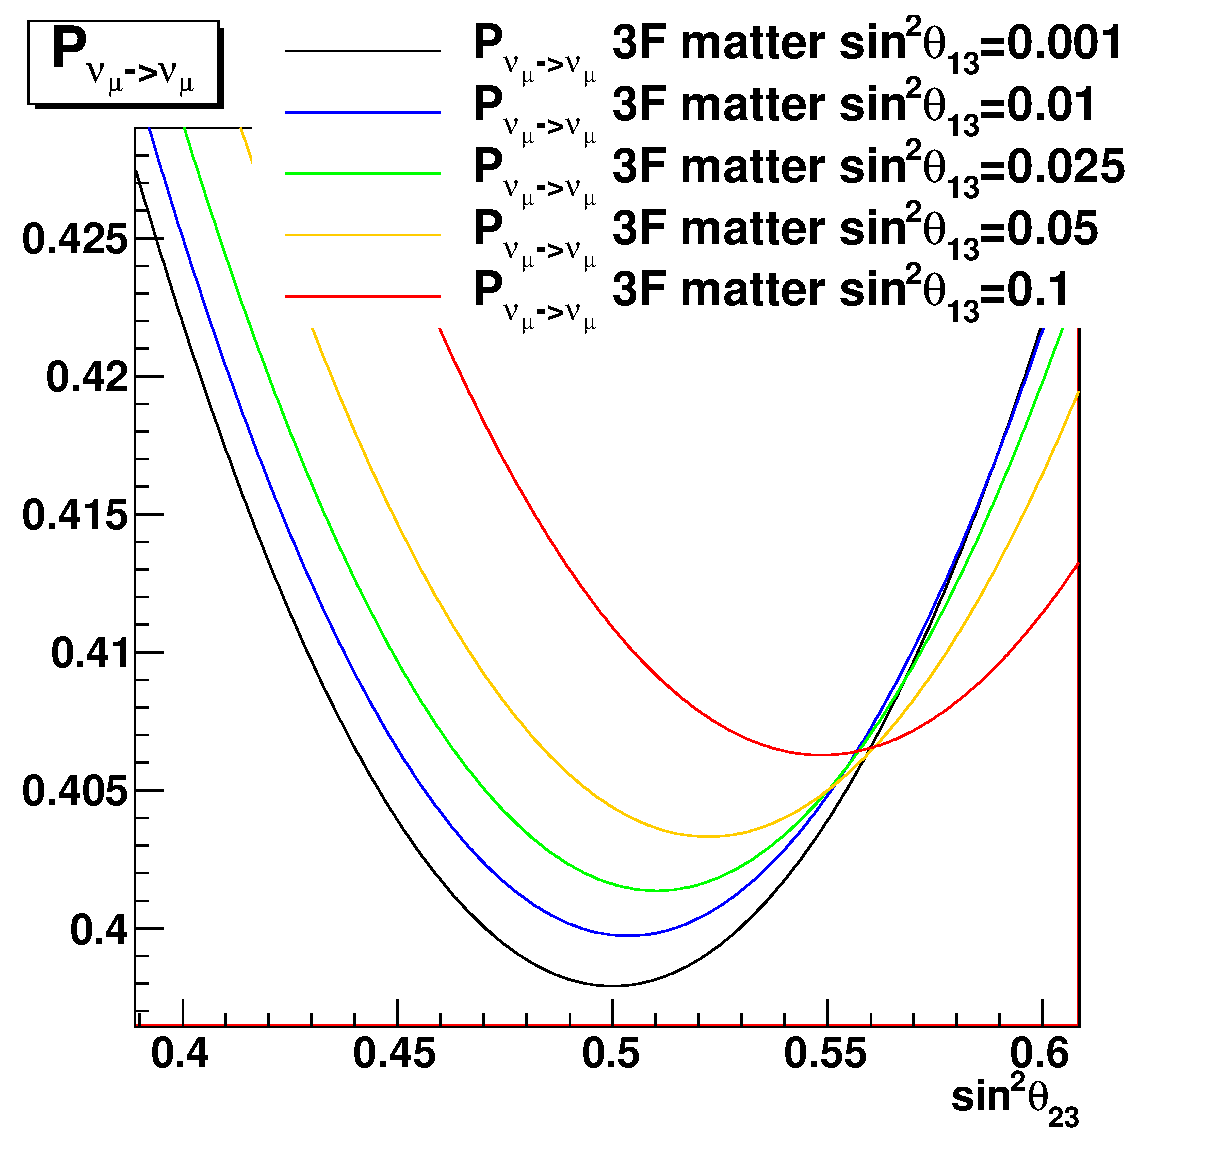
\includegraphics[width=0.5\textwidth]{images/appendix/theta23_symmetry/NuMuOscProbMatterSeveralValuesMix13Inverted.eps}
\caption{The 3-flavour P($\nu_{\mu}\rightarrow\nu_{\mu}$) with matter effects as a function of $\sin^{2}\theta_{23}$ for different values of 
$\sin^{2}\theta_{13}$ for the normal mass hierarchy (left) and the inverted mass hierarchy (right); $|\Delta m_{32}^{2}|$ is fixed to 2.4$\times$10$^{-3}$ 
eV$^{2}$/c$^{4}$ and $\delta_{CP}$ is fixed to 0.}
\label{fig:oscprobdifftheta13}
\end{center}
\end{figure}

\begin{equation}
\begin{array}{r}
P(\nu_{\mu}\rightarrow\nu_{\mu}) = 1 - 4 |U_{\mu 2}|^{2} |U_{\mu 1}|^{2} sin^{2}\left(\frac{\Delta m_{21}^{2} L}{4E}\right)\\
- 4 |U_{\mu 3}|^{2} |U_{\mu 1}|^{2} sin^{2}\left(\frac{\Delta m_{31}^{2} L}{4E}\right)\\
- 4 |U_{\mu 3}|^{2} |U_{\mu 2}|^{2} sin^{2}\left(\frac{\Delta m_{32}^{2} L}{4E}\right)
\end{array}
\label{eq:numusurv3f}
\end{equation}
where from equation \ref{eq:PMNSmatrix} the PMNS matrix elements are

\begin{equation}
\begin{array}{l}
|U_{\mu 1}|^{2} = s_{12}^{2} c_{23}^{2} +  s_{13}^{2}  s_{23}^{2}  c_{12}^{2} + 2  s_{12}s_{13}s_{23} c_{12}c_{23}cos(\delta)\\
|U_{\mu 2}|^{2} = c_{12}^{2} c_{23}^{2} +  s_{13}^{2}  s_{23}^{2}  s_{12}^{2} - 2  s_{12}s_{13}s_{23} c_{12}c_{23}cos(\delta)\\
|U_{\mu 3}|^{2} = s_{23}^{2}c_{13}^{2}
\end{array}
\label{eq:numusurv3felements}
\end{equation}


The movement of the center of symmetry can be explained mathematically by making some approximations to the 3-flavour P($\nu_{\mu}\rightarrow\nu_{\mu}$) in equation \ref{eq:numusurv3f}. 
Neglecting $\Delta m_{21}^{2}$, and therefore setting $\Delta m_{32}^{2} \approx \Delta m_{31}^{2}$, the third terms in $|U_{\mu 1}|^{2}$ and $|U_{\mu 2}|^{2}$ cancel each other,
\begin{equation}
\begin{split}
P(\nu_{\mu}\rightarrow\nu_{\mu}) &\approx 1 - 4 \sin^{2}\left(\frac{\Delta m_{31}^{2} L}{4E}\right) c_{13}^{2}s_{23}^{2} \left[ s_{12}^{2}c_{23}^{2}+c_{12}^{2}s_{13}^{2}s_{23}^{2}+c_{12}^{2}c_{23}^{2}+s_{12}^{2}s_{13}^{2}s_{23}^{2}\right] \\
&= 1 - 4 \sin^{2}\left(\frac{\Delta m_{31}^{2} L}{4E}\right) c_{13}^{2}s_{23}^{2} \left(s_{12}^{2} + c_{12}^{2} \right) \left[ c_{23}^{2} + s_{13}^{2}s_{23}^{2} \right] \\
&= 1 - 4 \sin^{2}\left(\frac{\Delta m_{31}^{2} L}{4E}\right) c_{13}^{2}s_{23}^{2} \left[ c_{23}^{2} + s_{13}^{2}s_{23}^{2}\right]
\end{split}
\label{numusurv3fapprox}
\end{equation}
Equation \ref{numusurv3fapprox} can be written as

\begin{equation}
y \approx 1-4Ax(1-k)\left[(1-x)+kx\right] = 1-4Ax(1-k) +4Ax^{2}(1-k)^{2}
\end{equation}
where A = $\sin^{2}\left(\frac{\Delta m_{31}^{2} L}{4E}\right)$, x = $s_{23}^{2}$ = $\sin^{2}(\theta_{23})$ and k = $s_{13}^{2}$ = $\sin^{2}(\theta_{13})$. 
The minimum of this equation can be found setting the first derivative to zero:

\begin{equation}
\frac{dy}{dx} = -4A(1-k) +8Ax(1-k)^{2}
\end{equation}
Since A $\neq$ 0 and (1-k) $\neq$ 0 (for an angle $\theta_{13}<\pi/2$), the value of x at which the oscillation probability is at a minimum is

\begin{equation}
x_{min} = \frac{1}{2(1-k)}
\label{xmin}
\end{equation}
It is clear from equation \ref{xmin} that x$_{min}$ is at $\frac{1}{2}$ when $\sin^{2}(\theta_{13})$ = 0. Also the only physically-allowed values of 
$\sin^{2}(\theta_{13})$ are $\geq$ 0, and this means that x$_{min}$ is at $\sin^{2}(\theta_{23}) > \frac{1}{2}$ when $\sin^{2}(\theta_{13})$ is non-zero. 
This simple result explains the dependence on $\sin^{2}(\theta_{13})$ of the center of symmetry of the P($\nu_{\mu}\rightarrow\nu_{\mu}$) curve,
and therefore the dependence on $\sin^{2}(\theta_{13})$ of the center of symmetry between the two minima of the $\Delta \chi^{2}$ 
distribution when plotted against $\sin^{2}(\theta_{23})$. 

As the true value of $\sin^{2}(\theta_{23})$ approaches the center of symmetry, the two minima become more difficult to separate.  If the true value of $\sin^{2}(\theta_{23})$ is exactly at the center of symmetry, there is only a single minimum in the distribution of $\Delta \chi^{2}$ against $\sin^{2}(\theta_{23})$. For a value of  $\sin^{2}(\theta_{23})$ close to the center of symmetry, the $\chi^{2}$ distribution becomes smoothed around the center of symmetry when statistical fluctuations are added, and the two minima disappear ending up in a single larger minimum combination of both (see for example Fig. \ref{fig:sensitivity:point0:dchisq_sinsqtheta23} ). This is the explanation of the bias observed in the distribution of residuals for $\sin^{2}(\theta_{23})$ for any oscillation point with true input value $\sin^{2}(\theta_{23}) = 0.5$ in Sec. \ref{app:fitter_performance}.

Usually one of the minima is in each octant, but it is also possible that both minima could be in the second octant. For example, the center of symmetry is at $\sin^{2}(\theta_{23})\approx0.513$ if $\sin^{2}(\theta_{13})\approx 0.025$ (from reactor experiments). If the best fit is very close to this center of symmetry, say at $\sin^{2}(\theta_{23})$ = 0.505, the second minimum is at $\sin^{2}(\theta_{23})$ = 0.521, i.e.\ both minima are in the second octant. 

As observed in Tab.\ \ref{tab:data_fits:best_fit_values}, the best-fit value for $\sin^{2}\theta_{23}$ is the same in both hierarchies 
although the best-fit values for the other oscillation parameters are different.
Already in Fig. \ref{fig:oscprobdifftheta13} one can see that the bias in $\sin^{2}\theta_{23}$ with respect to 0.5 at the center of symmetry of the P($\nu_{\mu}\rightarrow\nu_{\mu}$) curve 
is different for same values of $\sin^{2}\theta_{13}$ depending on the mass hierarchy selected (being the difference with 0.5 smaller for Inverted Hierarchy). 
Figure \ref{fig:oscprobbf} shows the  3-flavour P($\nu_{\mu}\rightarrow\nu_{\mu}$) oscillation probability with matter effects as a function of $\sin^{2}\theta_{23}$ for the best-fit
value found for Run1+2+3 dataset with Normal (left) and Inverted (right) Hierarchy. In this figure it is clear that the minimum is found at the best-fit value $\sin^{2}\theta_{23} = 0.516$
(indicated with a green line) in both hierarchies. 

\begin{figure}[htbp]
\begin{center}
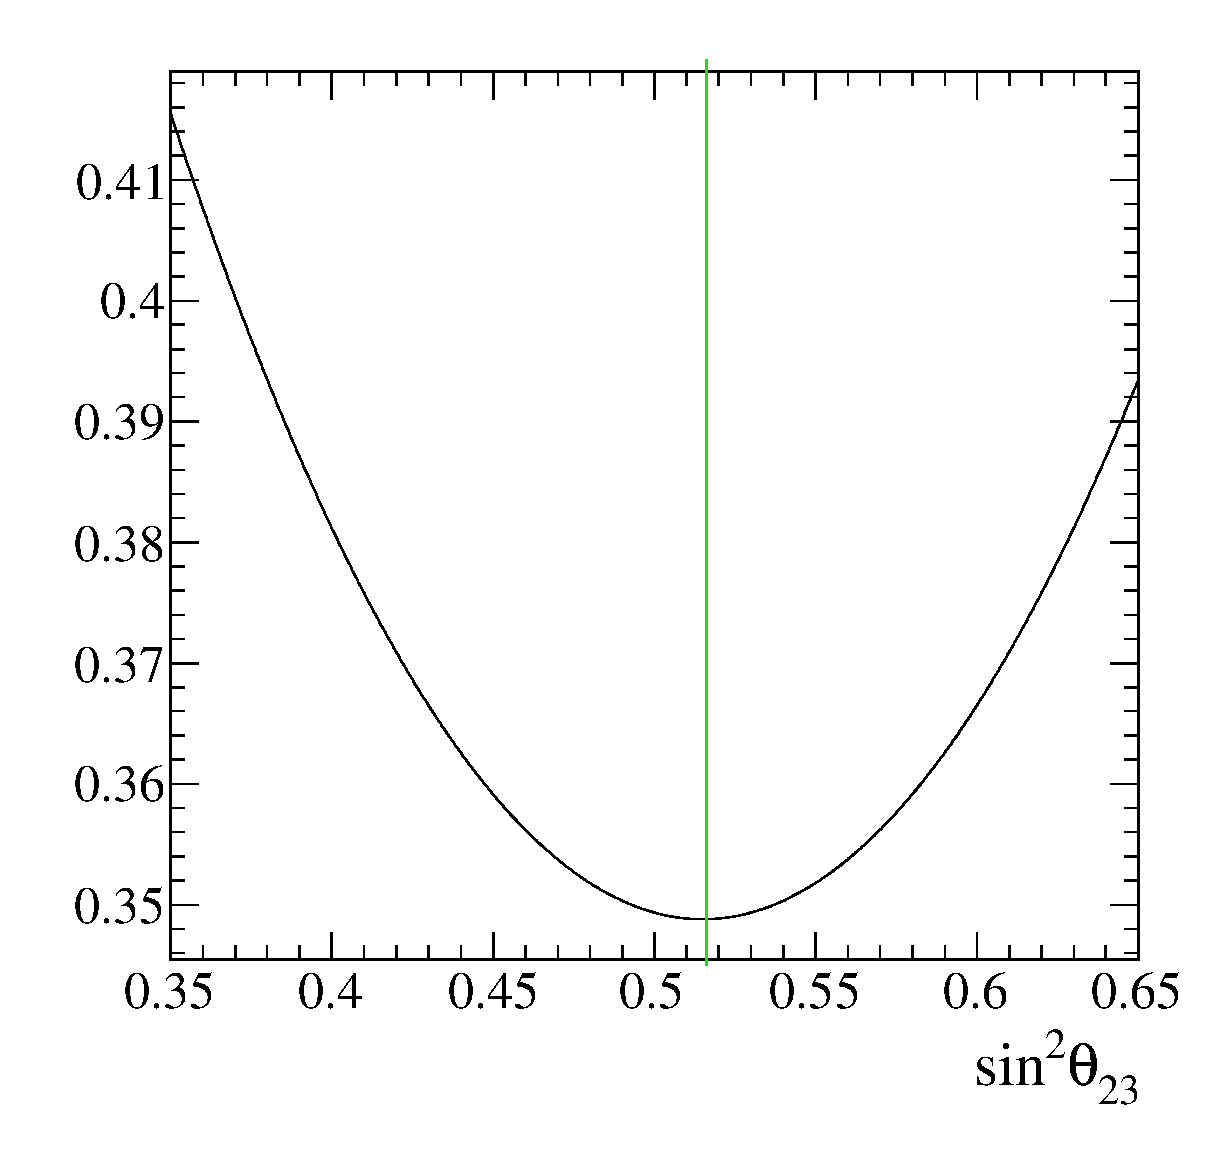
\includegraphics[width=0.5\textwidth]{images/appendix/theta23_symmetry/NuMuProbBFRun123NH.eps}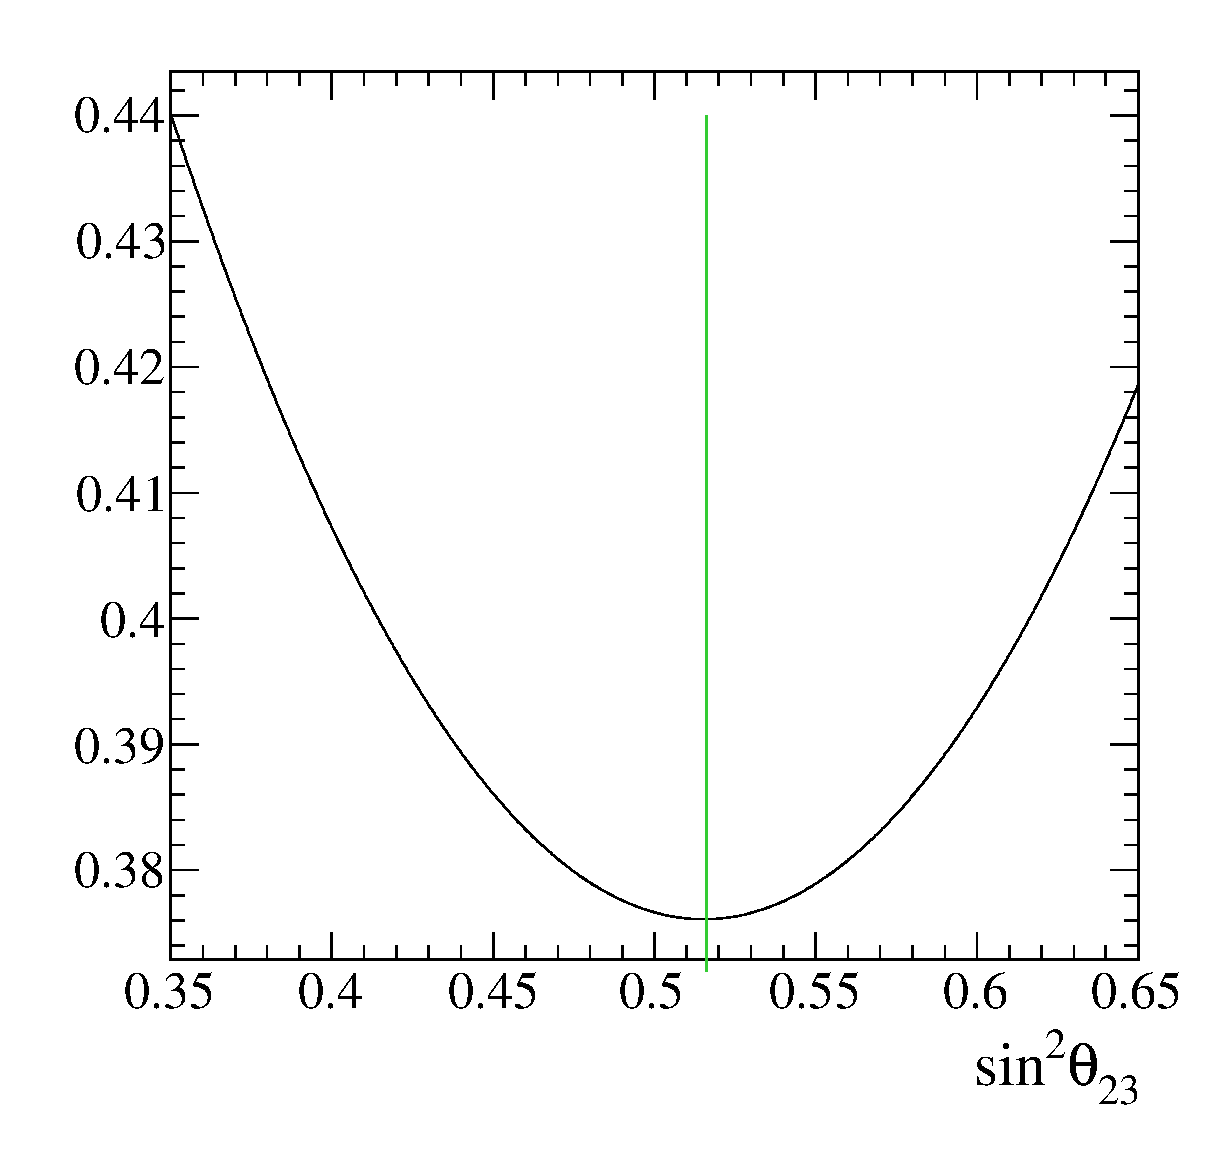
\includegraphics[width=0.5\textwidth]{images/appendix/theta23_symmetry/NuMuProbBFRun123IH.eps}
\caption{The 3-flavour P($\nu_{\mu}\rightarrow\nu_{\mu}$) with matter effects as a function of $\sin^{2}\theta_{23}$ for the best fit value found for
Run1+2+3 dataset fit with Normal Hierarchy (left) and Inverted Hierarchy (right). 
The values for the left plot are: $\sin^{2}\theta_{13} = 0.029$, $|\Delta m_{32}^{2}| = 2.494\times$10$^{-3}$ 
eV$^{2}$/c$^{4}$ and $\delta_{CP} = 2.086$.
The values for the right plot are: $\sin^{2}\theta_{13} = 0.034$, $|\Delta m_{32}^{2}| = 2.468\times$10$^{-3}$ 
eV$^{2}$/c$^{4}$ and $\delta_{CP} = 0.921$.
In both hierarchies the minimum is found at the best-fit value $\sin^{2}\theta_{23} = 0.516$
(indicated with a green line).}
\label{fig:oscprobbf}
\end{center}
\end{figure}


